\documentclass[11pt, a4paper]{article}

\usepackage[margin=1in]{geometry} %for mergin
\usepackage{graphicx}
\usepackage{fontawesome5}
\usepackage{float} % to use H, in figure positioning

%make macros for calculator
\newcommand{\calculator}{\faCalculator}

\begin{document}
\textbf{Critical Thinking Question:}

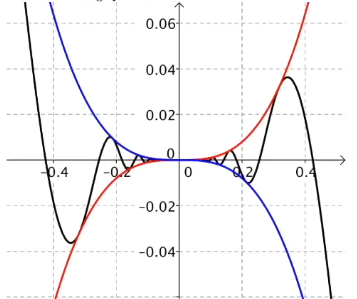
\includegraphics[scale = 0.8]{limit2.png}
\vspace{1in}
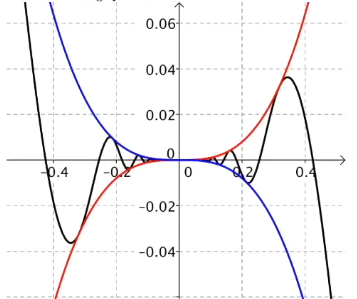
\includegraphics[height = 1in, width = 1in]{limit2.png}
Using Custom Height, Width:
\vspace{1in}
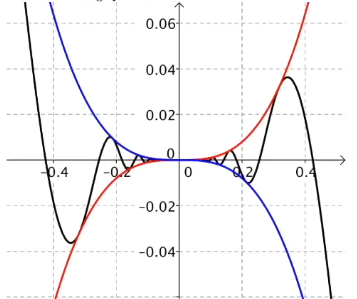
\includegraphics[width = 0.5 \textwidth]{limit2.png}

% Image in Center


\textbf{Image}
\begin{figure}[H]
    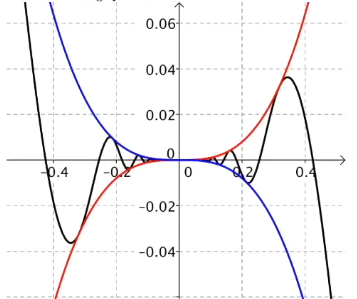
\includegraphics[scale=1]{limit2.png}
\end{figure}

\begin{enumerate}
    \item \faPen\ Pen
    \item \faEdit\ Notebook
    \item \calculator\ What’s	better	than	one	model	making	predictions?	Well,	how	about	a	bunch	of
 them?	Ensembling	is	a	technique	that	is	fairly	common
\end{enumerate}

% center the image also the caption of image
\begin{figure}[H]
    \centering
    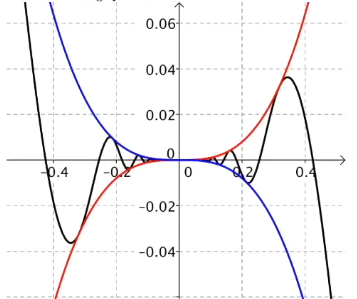
\includegraphics[scale=1]{limit2.png}
    \caption{The Squeeze Theorem}
\end{figure}








\end{document}